% Options for packages loaded elsewhere
\PassOptionsToPackage{unicode}{hyperref}
\PassOptionsToPackage{hyphens}{url}
%
\documentclass[
  american,
  man,floatsintext]{apa7}
\usepackage{amsmath,amssymb}
\usepackage{lmodern}
\usepackage{ifxetex,ifluatex}
\ifnum 0\ifxetex 1\fi\ifluatex 1\fi=0 % if pdftex
  \usepackage[T1]{fontenc}
  \usepackage[utf8]{inputenc}
  \usepackage{textcomp} % provide euro and other symbols
\else % if luatex or xetex
  \usepackage{unicode-math}
  \defaultfontfeatures{Scale=MatchLowercase}
  \defaultfontfeatures[\rmfamily]{Ligatures=TeX,Scale=1}
\fi
% Use upquote if available, for straight quotes in verbatim environments
\IfFileExists{upquote.sty}{\usepackage{upquote}}{}
\IfFileExists{microtype.sty}{% use microtype if available
  \usepackage[]{microtype}
  \UseMicrotypeSet[protrusion]{basicmath} % disable protrusion for tt fonts
}{}
\makeatletter
\@ifundefined{KOMAClassName}{% if non-KOMA class
  \IfFileExists{parskip.sty}{%
    \usepackage{parskip}
  }{% else
    \setlength{\parindent}{0pt}
    \setlength{\parskip}{6pt plus 2pt minus 1pt}}
}{% if KOMA class
  \KOMAoptions{parskip=half}}
\makeatother
\usepackage{xcolor}
\IfFileExists{xurl.sty}{\usepackage{xurl}}{} % add URL line breaks if available
\IfFileExists{bookmark.sty}{\usepackage{bookmark}}{\usepackage{hyperref}}
\hypersetup{
  pdftitle={Study 4},
  pdfauthor={Blinded1, Blinded2, Blinded1, \& Blinded1},
  pdflang={en-US},
  pdfkeywords={keywords},
  hidelinks,
  pdfcreator={LaTeX via pandoc}}
\urlstyle{same} % disable monospaced font for URLs
\usepackage{graphicx}
\makeatletter
\def\maxwidth{\ifdim\Gin@nat@width>\linewidth\linewidth\else\Gin@nat@width\fi}
\def\maxheight{\ifdim\Gin@nat@height>\textheight\textheight\else\Gin@nat@height\fi}
\makeatother
% Scale images if necessary, so that they will not overflow the page
% margins by default, and it is still possible to overwrite the defaults
% using explicit options in \includegraphics[width, height, ...]{}
\setkeys{Gin}{width=\maxwidth,height=\maxheight,keepaspectratio}
% Set default figure placement to htbp
\makeatletter
\def\fps@figure{htbp}
\makeatother
\setlength{\emergencystretch}{3em} % prevent overfull lines
\providecommand{\tightlist}{%
  \setlength{\itemsep}{0pt}\setlength{\parskip}{0pt}}
\setcounter{secnumdepth}{-\maxdimen} % remove section numbering
% Make \paragraph and \subparagraph free-standing
\ifx\paragraph\undefined\else
  \let\oldparagraph\paragraph
  \renewcommand{\paragraph}[1]{\oldparagraph{#1}\mbox{}}
\fi
\ifx\subparagraph\undefined\else
  \let\oldsubparagraph\subparagraph
  \renewcommand{\subparagraph}[1]{\oldsubparagraph{#1}\mbox{}}
\fi
% Manuscript styling
\usepackage{upgreek}
\captionsetup{font=singlespacing,justification=justified}

% Table formatting
\usepackage{longtable}
\usepackage{lscape}
% \usepackage[counterclockwise]{rotating}   % Landscape page setup for large tables
\usepackage{multirow}		% Table styling
\usepackage{tabularx}		% Control Column width
\usepackage[flushleft]{threeparttable}	% Allows for three part tables with a specified notes section
\usepackage{threeparttablex}            % Lets threeparttable work with longtable

% Create new environments so endfloat can handle them
% \newenvironment{ltable}
%   {\begin{landscape}\begin{center}\begin{threeparttable}}
%   {\end{threeparttable}\end{center}\end{landscape}}
\newenvironment{lltable}{\begin{landscape}\begin{center}\begin{ThreePartTable}}{\end{ThreePartTable}\end{center}\end{landscape}}

% Enables adjusting longtable caption width to table width
% Solution found at http://golatex.de/longtable-mit-caption-so-breit-wie-die-tabelle-t15767.html
\makeatletter
\newcommand\LastLTentrywidth{1em}
\newlength\longtablewidth
\setlength{\longtablewidth}{1in}
\newcommand{\getlongtablewidth}{\begingroup \ifcsname LT@\roman{LT@tables}\endcsname \global\longtablewidth=0pt \renewcommand{\LT@entry}[2]{\global\advance\longtablewidth by ##2\relax\gdef\LastLTentrywidth{##2}}\@nameuse{LT@\roman{LT@tables}} \fi \endgroup}

% \setlength{\parindent}{0.5in}
% \setlength{\parskip}{0pt plus 0pt minus 0pt}

% Overwrite redefinition of paragraph and subparagraph by the default LaTeX template
% See https://github.com/crsh/papaja/issues/292
\makeatletter
\renewcommand{\paragraph}{\@startsection{paragraph}{4}{\parindent}%
  {0\baselineskip \@plus 0.2ex \@minus 0.2ex}%
  {-1em}%
  {\normalfont\normalsize\bfseries\itshape\typesectitle}}

\renewcommand{\subparagraph}[1]{\@startsection{subparagraph}{5}{1em}%
  {0\baselineskip \@plus 0.2ex \@minus 0.2ex}%
  {-\z@\relax}%
  {\normalfont\normalsize\itshape\hspace{\parindent}{#1}\textit{\addperi}}{\relax}}
\makeatother

% \usepackage{etoolbox}
\makeatletter
\patchcmd{\HyOrg@maketitle}
  {\section{\normalfont\normalsize\abstractname}}
  {\section*{\normalfont\normalsize\abstractname}}
  {}{\typeout{Failed to patch abstract.}}
\patchcmd{\HyOrg@maketitle}
  {\section{\protect\normalfont{\@title}}}
  {\section*{\protect\normalfont{\@title}}}
  {}{\typeout{Failed to patch title.}}
\makeatother
\keywords{keywords\newline\indent Word count: TBC}
\usepackage{csquotes}
\ifxetex
  % Load polyglossia as late as possible: uses bidi with RTL langages (e.g. Hebrew, Arabic)
  \usepackage{polyglossia}
  \setmainlanguage[variant=american]{english}
\else
  \usepackage[main=american]{babel}
% get rid of language-specific shorthands (see #6817):
\let\LanguageShortHands\languageshorthands
\def\languageshorthands#1{}
\fi
\ifluatex
  \usepackage{selnolig}  % disable illegal ligatures
\fi
\newlength{\cslhangindent}
\setlength{\cslhangindent}{1.5em}
\newlength{\csllabelwidth}
\setlength{\csllabelwidth}{3em}
\newenvironment{CSLReferences}[2] % #1 hanging-ident, #2 entry spacing
 {% don't indent paragraphs
  \setlength{\parindent}{0pt}
  % turn on hanging indent if param 1 is 1
  \ifodd #1 \everypar{\setlength{\hangindent}{\cslhangindent}}\ignorespaces\fi
  % set entry spacing
  \ifnum #2 > 0
  \setlength{\parskip}{#2\baselineskip}
  \fi
 }%
 {}
\usepackage{calc}
\newcommand{\CSLBlock}[1]{#1\hfill\break}
\newcommand{\CSLLeftMargin}[1]{\parbox[t]{\csllabelwidth}{#1}}
\newcommand{\CSLRightInline}[1]{\parbox[t]{\linewidth - \csllabelwidth}{#1}\break}
\newcommand{\CSLIndent}[1]{\hspace{\cslhangindent}#1}

\title{Study 4}
\author{Blinded\textsuperscript{1}, Blinded\textsuperscript{2}, Blinded\textsuperscript{1}, \& Blinded\textsuperscript{1}}
\date{}


\shorttitle{Cognitive Load and Moral Dumbfounding}

\authornote{

Correspondence concerning this article should be addressed to Blinded, Blinded. E-mail: Blinded

}

\affiliation{\vspace{0.5cm}\textsuperscript{1} Blinded\\\textsuperscript{2} Blinded}

\abstract{
Six studies etc.
}



\begin{document}
\maketitle

\hypertarget{study-4---online-replication-3}{%
\section{Study 4 - Online Replication 3}\label{study-4---online-replication-3}}

Study 3 found a significant relationship between cognitive load and response to the critical slide and a significant relationship between Need for Cognition and response to the critical slide. The aim of Study 4 was to replicate these findings. In addition Study 4 included a manipulation check to assess the effectiveness of the cognitive load manipulation employed.

\hypertarget{study-4-method}{%
\subsection{Study 4: Method}\label{study-4-method}}

\hypertarget{study-4-participants-and-design}{%
\subsubsection{Study 4: Participants and Design}\label{study-4-participants-and-design}}

Study 4 was a between subjects design. The dependent variable was response to the critical slide. The independent variable was cognitive load with two levels: present and absent. Need for Cognition (Cacioppo \& Petty, 1982; Petty, Cacioppo, \& Kao, 1984) was included as a potential correlate and moderator variable.

Following the elimination of 29 participants who scored less than 7 on the memory task we were left with a final sample of 127 participants (84 female, 43 male; \emph{M}\textsubscript{age} = 41.19, min = 21, max = 74, \emph{SD} = 13.91). Participants in this sample were recruited through
MTurk (under the same conditions as Studies 2 and 3).

\hypertarget{study-4-procedure-and-materials}{%
\subsubsection{Study 4: Procedure and Materials}\label{study-4-procedure-and-materials}}

Study 4 was the same as Study 3 with one change, the inclusion of a manipulation check. A prose paragraph was included after participants made their revised judgements. Participants were then asked three comprehension questions relating to the prose paragraph. It was expected that participants in the control group would perform better at this task than participants under cognitive load (Just \& Carpenter, 1992).

\hypertarget{study-4-results}{%
\subsection{Study 4: Results}\label{study-4-results}}

Ninety eight participants (77.17\%) rated the behavior of Julie and Mark as wrong initially, and ninety two participants (72.44\%) rated the behavior as wrong at the end of the task. Initial ratings (\emph{M} = 2.09, \emph{SD} = 1.62) were significantly more severe than revised ratings (\emph{M} = 2.31, \emph{SD} = 1.79), \emph{t}(126) = -3.14, \emph{p} = .002; \emph{d} = 0.28. Inspection of the binned judgments revealed that thirteen participants changed the valence of their judgments, and all but two of these involved one judgment that was neutral (see Supplementary materials Table XX).

\begin{figure}
\centering
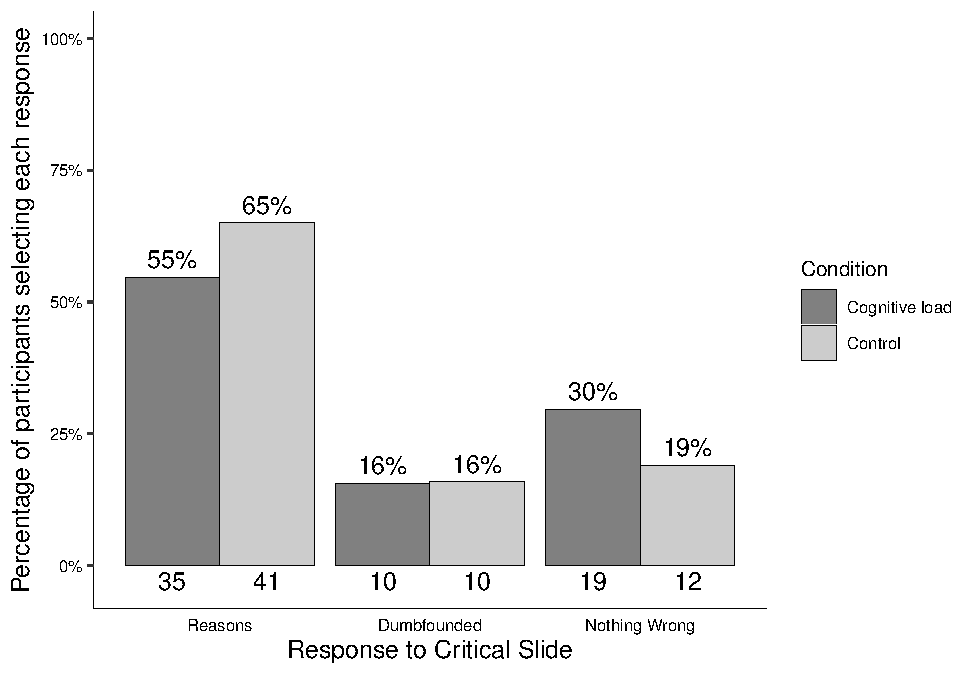
\includegraphics{Study_4_files/figure-latex/ch5S4fig2criticalcondition-1.pdf}
\caption{\label{fig:ch5S4fig2criticalcondition}Study 4: Responses to critical slide for the cognitive load group (\emph{N} = 64) and the control group (\emph{N} = 61)}
\end{figure}

Investigation of the responses to the manipulation check questions revealed no difference in the number of correct answers to these questions between the cognitive load group and the control group \emph{t}(123.91) = 0.57, \emph{p} = .569; \emph{d} = 0.10. There was also no difference in time taken to read the vignette between the groups \emph{t}(63.40) = 1.62, \emph{p} = .111; \emph{d} = 0.28.

On the critical slide, twenty participants (15.75\%) selected ``It's wrong but I can't think of a reason.'' Seventy six participants (59.84\%) selected ``It's wrong and I can provide a valid reason''; and thirty one participants (24.41\%) selected ``There is nothing wrong.''

\begin{table}[tbp]

\begin{center}
\begin{threeparttable}

\caption{\label{tab:S4tab1dumb}Study 4 – Observed counts, expected counts, and standardised residuals for each response to the critical slide depending on cognitive load}

\begin{tabular}{llcc}
\toprule
 & \multicolumn{1}{c}{} & \multicolumn{1}{c}{Cognitive Load} & \multicolumn{1}{c}{Control}\\
\midrule
Observed count & Reasons & 35.00 & 41.00\\
 & Dumbfounded & 10.00 & 10.00\\
 & Nothing Wrong & 19.00 & 12.00\\
Expected count & Reasons & 38.30 & 37.70\\
 & Dumbfounded & 10.08 & 9.92\\
 & Nothing Wrong & 15.62 & 15.38\\
Standardised residuals & Reasons & -1.19 & 1.19\\
 & Dumbfounded & -0.04 & 0.04\\
 & Nothing Wrong & 1.40 & -1.40\\
\bottomrule
\addlinespace
\end{tabular}

\begin{tablenotes}[para]
\normalsize{\textit{Note.} * = sig. at \emph{p} < .05; ** = sig. at \emph{p} < .001}
\end{tablenotes}

\end{threeparttable}
\end{center}

\end{table}

A chi-squared test for independence revealed no significant association between experimental condition and response to the critical slide, \(\chi\)\textsuperscript{2}(2, \emph{N} = 127) = 2.05, \emph{p} = .359, \emph{V} = 0.13, the observed power was 0.23. The responses to the critical slide for the experimental group (\emph{N} = 64) and the control group (\emph{N} = 63) are displayed in Figure~\ref{fig:ch5S4fig2criticalcondition}. The observed counts, expected counts and standardised residuals are displayed in Table~\ref{tab:S4tab1dumb}.

A multinomial logistic regression revealed no statistically significant association between Need for Cognition and response to the critical slide, \(\chi\)\textsuperscript{2}(2, \emph{N} = 127) = 1.5, \emph{p} = .472, the observed power was 0.18 (see Supplamentary Figure XX for relative probabilities of selecting each response depending on Need for Cognition).

\hypertarget{refs}{}
\begin{CSLReferences}{1}{0}
\leavevmode\hypertarget{ref-cacioppo_need_1982}{}%
Cacioppo, J. T., \& Petty, R. E. (1982). The need for cognition. \emph{Journal of Personality and Social Psychology}, \emph{42}(1), 116--131. \url{https://doi.org/10.1037/0022-3514.42.1.116}

\leavevmode\hypertarget{ref-just_capacity_1992}{}%
Just, M. A., \& Carpenter, P. A. (1992). A capacity theory of comprehension: Individual differences in working memory. \emph{Psychological Review}, \emph{99}(1), 122--149. \url{https://doi.org/10.1037/0033-295X.99.1.122}

\leavevmode\hypertarget{ref-petty_efficient_1984}{}%
Petty, R. E., Cacioppo, J. T., \& Kao, C. F. (1984). The efficient assessment of need for cognition. \emph{Journal of Personality Assessment}, \emph{48}(3), 306--307.

\end{CSLReferences}


\end{document}
